\subsection{PICARD - Parsing Incrementally for Constrained Auto-Regressive Decoding} \label{picard}

PICARD\cite{Scholak2021:PICARD} stands for "Parsing Incrementally for Constrained Auto-Regressive Decoding.". It can be used with any existing language model decoder or vocabulary based on auto-regressive language modeling.

PICARD allows for the generation of executable code by constraining the output of the language model to be syntactically and semantically correct.

It does this by integrating with standard beam search, a technique used in natural language processing to generate a sequence of words or tokens by expanding a beam of hypotheses step by step. At each decoding step, PICARD checks whether the most likely tokens are valid and if not, it discards them. PICARD is compatible with any model that generates a sequence of tokens and can be used with character, subword, and word-level language models without requiring exceptional recovery.

It effectively improves the performance of existing models and achieves state-of-the-art performance on tasks such as text-to-SQL translation.
Warps model prediction scores and integrates trivially with existing greedy and beam search algorithms used in auto-regressive decoding from language models.

At each generation step, Picard first restricts prediction to the top-k highest probability tokens and then assigns a score of negative infinity to those that fail Picard's numerous checks.

Four Picard mode settings control their comprehensiveness: off (no checking), lexing, parsing without guards and parsing with guards-the highest mode.

Picard can detect spelling errors in keywords or reject table and column names that are invalid for the given SQL schema.
"Out-of-distribution compositional generalization and natural language variation" refers to the ability of a natural language processing (NLP) system to handle novel combinations of words and phrases that it has not seen before while also being able to handle variations in language usage.
Compositional generalization refers to the ability of an NLP system to understand and generate novel combinations of words and phrases by using its knowledge of the meanings and relationships of individual words and phrases. This is an essential aspect of NLP because it allows the system to understand and generate language flexibly and adaptively.

Natural language variation refers to the fact that there are many different ways that people can express the same ideas or concepts in natural language. This can be due to differences in dialect, style, or tone, and it can make it challenging for an NLP system to understand and generate language accurately.

Together, out-of-distribution compositional generalization and natural language variation represent fundamental challenges in the field of NLP. They require NLP systems to handle a wide range of language input and output in order to be effective.

As an optional feature, Picard can be enabled at inference time and is absent from pre-training or fine-tuning. In the case of text-to-SQL translation, Picard operates directly on the output of the language model.
Picard demonstrates state-of-the-art performance on challenging Spider and CoSQL text-to-SQL translation tasks.

Picard warps model prediction scores and integrates trivially with existing greedy and beam search algorithms. In addition to the token ids of the current hypothesis, the model's language modeling head also predicts the log-softmax scores for each vocabulary token. Additionally, Picard has access to SQL schema information, including table and column names and which column resides in which table.

Motivated by the success of Shaw et al. (2021), who demonstrated that a pre-trained T5-Base or T5-3B model could effectively learn the text-to-SQL task, generalize to never-before-seen databases, and even rival the state-of-the-art methods of Choi et al. (2021) and Wang et al. (2020) without any modifications to the model itself, the researchers opted to use T5 as the baseline for all their experiments. The results from Shaw et al. (2021) suggest that T5-based models had the potential to improve the field of natural language processing significantly. Therefore, the researchers sought to take advantage of the capabilities of T5 in order to gain new insights into how natural language can be effectively utilized to solve complex tasks.

\subsubsection{Beam Search}

\begin{figure}[h]
    \centering
    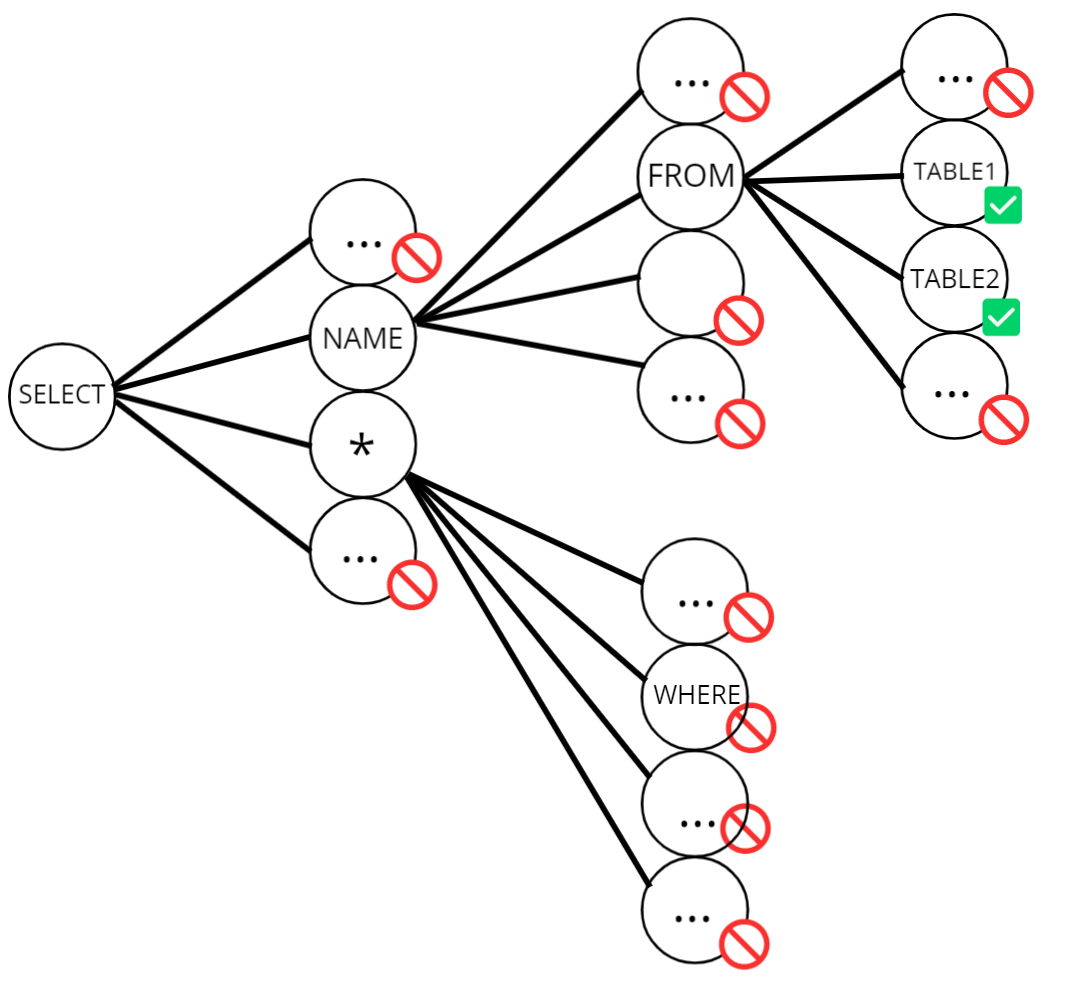
\includegraphics[width=0.5\textwidth]{pics/picard/beam.png}
    \caption{Beam Search}
    \label{fig:beam_search}
\end{figure}

Beam search is a widely used search algorithm in natural language processing and machine learning. It is beneficial in sequence-to-sequence (seq2seq) models, which generate output sequences based on input sequences. Beam search is used to find the most likely sequence of output words given an input sequence.
\\
The basic idea behind beam search is to maintain a set of the most likely sequences at each step of the decoding process. This set of sequences, called the "beam," is initially set to the starting point of the decoding process, and at each step, new sequences are generated by considering all the following possible words. The new sequences are then ranked based on their likelihood, and the highest-ranking sequences are added to the beam. The process is repeated until a stopping criterion is met \cite{10.1371/journal.pone.0211558}.
Beam search is handy in seq2seq models because it allows the model to generate multiple output sequences rather than just a single sequence. This is important because, in many cases, there may be multiple valid outputs for a given input sequence. By generating multiple outputs, beam search allows the model to explore the space of possible outputs and find the most likely sequences.
\\
One of the critical advantages of beam search is that it is computationally efficient. Because it only considers a small number of sequences at each step, it can quickly find the most likely sequences without exploring the entire space of possible outputs. This makes it well-suited for use in applications with limited computational resources, such as on mobile devices or in real-time systems.
Another advantage of beam search is that it can be used with other techniques, such as attention mechanisms, to improve the performance of seq2seq models. Attention mechanisms allow the model to focus on specific parts of the input sequence when generating the output, which can help to improve the quality of the generated sequences.
\\
In conclusion, Beam Search is a robust algorithm widely used in natural language processing and machine learning, particularly in the context of sequence-to-sequence (seq2seq) models. It allows the model to generate multiple output sequences rather than just a single sequence and is computationally efficient, making it well-suited for use in applications where computational resources are limited. Additionally, it can be combined with other techniques, such as attention mechanisms, to improve the performance of seq2seq models.

\subsubsection{DB Engines}

The Picard Method is a method for constrained inference on top of an existing model, but it is not a model itself. Currently, the PICARD parser and the supporting software are not supported for PostgreSQL, MySQL and others, which would require changes to the PICARD parser, translation of Spider databases and text-to-SQL data, and retraining models to produce MSSQL code. To use the Picard Method, a complex toolchain of Haskell code is built with CABAL and requires a complicated toolchain for the Facebook Thrift library.

After the setup, the Picard server can be started by running the compiled standalone executable PICARD. This executable is responsible for providing the necessary information to the user, such as specific parameters and options within the constrained inference. It is important to note that the Picard Method is not a full-fledged model; therefore, it is necessary to combine it with an existing model to get a complete inference system.

The thrift library is used for communication between the parser and the beam search algorithm. The parser, written in the efficient and powerful Haskell programming language, is used in combination with the hf transformers, which is a Python package. To further expand the scope of the system, new SQL engines can be supported by adding a parser for each one.

These parsers also need to be written in Haskell, as the existing SQLite parser is of limited use in this regard, as it has been written to work best on Spider's subset of SQLite and only supports part of the SQLite specification. This means that more advanced parsers must be created to maximize the system's capabilities.

Additionally, these parsers need to be written with a high level of precision in order to ensure that the system can effectively communicate with various engines and databases.